\section{Test}
\label{sec:Test}

Die zu erstellende Software ist mit Abschluss der Umsetzungsphase fertiggestellt und einsatzbereit. Vor Projektabschluss und -übergabe soll die Software auf ihre Qualität geprüft werden. Es soll darüber hinaus verifiziert werden, dass die Anforderungen des Lastenheftes umgesetzt wurden. Sowohl Qualität, als auch die Umsetzung der Anforderungen werden im Folgenden in einem zweistufigen Praxistest der Software sichergestellt.

Im ersten Schritt wird die Software einem Alphatest unterzogen. Ein Alphatest liegt immer dann vor, wenn die Tests von Personen durchgeführt werden, die an der Entwicklung eines Produktes beteiligt waren, in diesem Fall das Projektteam. In diesem Test werden vor allem die Produktfunktionen des Lastenheftes (siehe Abschnitt \nameref{sec:Lastenheft} auf Seite \pageref{sec:Lastenheft}) überprüft. In diesem Test sollen erste grobe Fehler in Bedienung, Anzeige und Verhalten gefunden werden und es soll zusätzlich sichergestellt werden, dass alle Anforderungen des Auftraggebers umgesetzt sind. Die Tests der Produktfunktionen werden zusätzlich in den vier führenden Browsern\footnote{Quelle: \url{http://www.chip.de}} durchgeführt, um browserübergreifende Funktionalität sicherzuestellen.
Dabei wurden jeweils die Testbereiche Bedienung, Anzeige und Verhalten unterschieden. Das Ergbeniss des durchgeführten Alphatests ist in nachfolgender \abbildung{Alphatest} festgehalten:

\begin{figure}[htb]
\centering
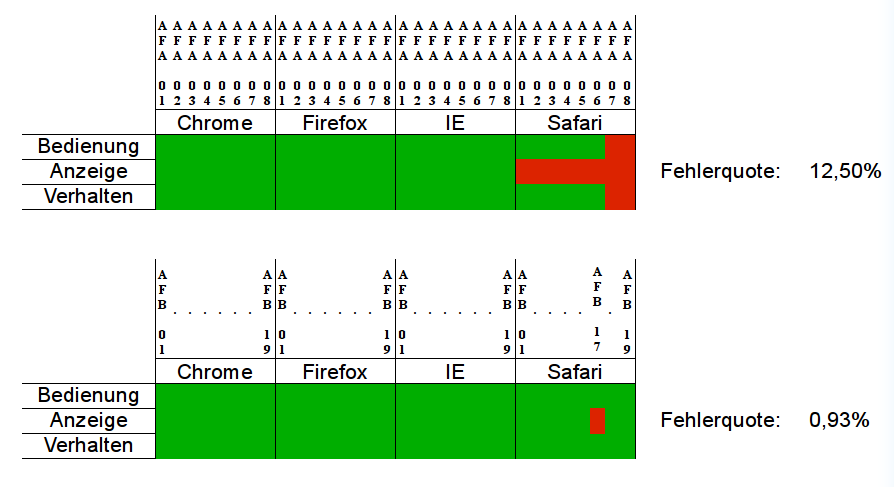
\includegraphics[width=1.0\textwidth]{Alphatest.png}
\caption[Mockup Backend]{Graphische Darstellung des Alphatests\protect\footnotemark}
\label{fig:Alphatest}
\end{figure}
\footnotetext{Quelle: Eigene Darstellung}

Die Auswertung des Alphatests zeigt, dass alle Anforderungen umgesetzt wurden und funktionsfähig sind. Darüber hinaus
traten in keinem der geprüften Anwendungsfälle Fehler auf.
Dagegen zeigten sich aber beim Vergleich der verschiedenen getesteten Browser deutliche Unterschiede in der
Darstellungsgeschwindkeit.
Die Möglichkeit sich in einzelnen Panoramafotos umzusehen stellte sich zum Beispiel im Google Chrome Browser
flüssiger dar als im Internet Explorer oder im Firefox-Browser. Es wird daher empfholen den Google Chrome Browser
zur Benutzung der Software zu verwenden.
Neben browserspezifischen Darstellungsunterschieden konnten in diesem Alphatest auch kleinere Schwachstellen und Fehler gefunden werden, die nicht in den Anwendungsfällen enthalten waren. So zum Beispiel die falsche Verlinkung einer Datei oder das Fehlen einer Sicherheitsabfrage beim Löschen eines Datensatzes. Diese Mängel wurden im Anschluss an den Alphatest direkt beseitigt.
Der Alphatest zeigt aus Sicht des Entwicklerteams den funktionalen Erfolg des Projektes.

Im zweiten Schritt der Testphase wird die Software einem Betatest unterzogen. Dieser Betatest wird von Personen
durchgeführt, die an der Entwicklung nicht beteiligt waren. Dieser Test wurde von dem Projektteam durchgeführt,
um weitere Fehler in der Software zu identfizieren und Projektziele zu verifizieren. Die Verfiktion der Projektziele
durch den Betatest ist dabei nicht primärer Gegenstand der vorliegenden Projektbetrachtung und wird daher
nicht weiter vertieft. Die Verifikation der Ziele kann in \citet{unternehmensfuehrung2014} nachgelesen werden.
Die Folgende Auflistung zeigt Fehler und Verbesserungsvorschläge, die von Betatestern geäußert wurden:

\begin{itemize}
  \item Ausführlichere Erklärungen zur Anwendung
  \item Optimierte Darstellung für mobile Endgeräte
  \item Einrichtung eines Hilfe Buttons
  \item Erstellung einer Übersichtskarte aus Vogelperspektive
  \item Einführung von Tastenkürzeln zum navigieren
\end{itemize}

Aufbauend auf diesem verkürzt dargestellten Feedback der Betatester wird ein weiterer Entwicklungszyklus begonnen, in dem
diese Kritik ausgebessert wird. Nicht jede Kritik kann dabei berücksichtigt werden. Die verbesserte Darstellung für
mobile Geräte kann zum Beispiel in diesem Projekt nicht mehr umgestetzt werden, da hierfür ein größerer
Entwicklungsaufwand nötig wäre.

Neben dieser Fehleranalyse wird analog zu dem Alphatest auch im Betatest ein besonderer Fokus auf den
Erfolg des Projektes aus Sicht der Betatester gelegt. Aus diesem Grund zeigt die folgende Grafik eine subjektive
Bewertung des Projektes aus Sicht der Betatester.

\begin{figure}[htb]
\centering
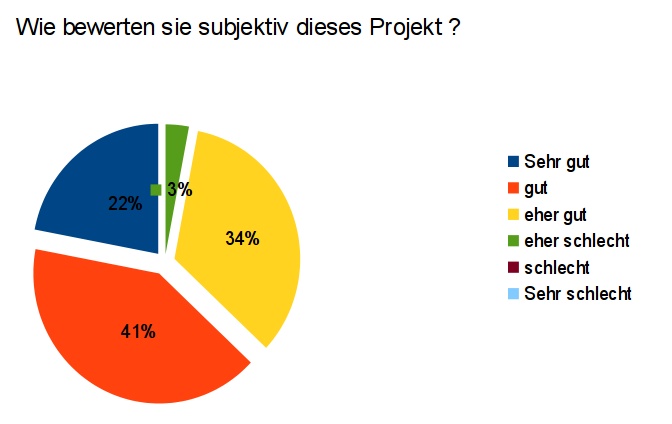
\includegraphics[width=1.0\textwidth]{Betatest.png}
\caption[Alphatest Auswertung]{Erfolg des Projektes aus Sicht der Betatester\protect\footnotemark}
\label{fig:Betatest}
\end{figure}
\footnotetext{Quelle: Eigene Darstellung}

Sowohl aus Sicht des Entwicklerteams, als auch aus Sicht der Betatester erfüllt das Projekt am Ende der Testphase
seine Funktion und erzielt darüber hinaus deutlich positive Resonanz.